\documentclass{beamer}
\usepackage[francais]{babel}
\usepackage[utf8]{inputenc} % Required for including letters with accents
\usepackage[T1]{fontenc} % Use 8-bit encoding that has 256 glyphs
\usepackage{pythontex}
\usepackage{amsthm}
\usepackage{amsmath}
\usepackage{amssymb}
\usepackage{mathrsfs}
\usepackage{graphicx}
\usepackage{geometry}
\usepackage{stmaryrd}
\usepackage{tikz} 
\usetikzlibrary{matrix,decorations.pathreplacing,calc,fit,backgrounds}
\usetikzlibrary{patterns}
%\usetikzlibrary{intersections}
\usepackage {mathtools} 
%%%%%%%%%%%%%%%

%\usepackage[latin1]{inputenc}
%\usepackage[T1]{fontenc}
%\usepackage[francais]{babel}

\usepackage[cache=false]{minted}
 \definecolor{darkWhite}{rgb}{0.94,0.94,0.94}
 \usepackage[cache=false]{minted}
\definecolor{LightGray}{gray}{0.9}
\definecolor{monOrange}{rgb}{0.97,0.35,0.04}

%%%%%%%%%%%%%%%


\usepackage{stmaryrd}
%\usepackage{tikz}
%\usetikzlibrary{tikzmark}
\usepackage{empheq}
\usepackage{longtable}
\usepackage{booktabs} 
\usepackage{array}
\usepackage{pstricks}
\usepackage{pst-3dplot}
\usepackage{pst-tree}
\usepackage{pstricks-add}
\usepackage{upgreek}
%\usepackage{epstopdf}
\usepackage{eolgrab}
\usepackage{chngpage}
 \usepackage{calrsfs}
 % Appel du package pythontex 
\usepackage{pythontex}

\usetikzlibrary{decorations.pathmorphing}
\def \de {{\rm d}}
\usepackage{color}
%\usepackage{xcolor}
%\usepackage{textcomp}
\newcommand{\mybox}[1]{\fbox{$\displaystyle#1$}}
\newcommand{\myredbox}[1]{\fcolorbox{red}{white}{$\displaystyle#1$}}
\newcommand{\mydoublebox}[1]{\fbox{\fbox{$\displaystyle#1$}}}
\newcommand{\myreddoublebox}[1]{\fcolorbox{red}{white}{\fcolorbox{red}{white}{$\displaystyle#1$}}}
\usetheme[options]{Boadilla}
\definecolor{purple2}{RGB}{153,0,153} % there's actually no standard purple
\definecolor{green2}{RGB}{0,153,0} % a darker green
\usepackage{xcolor}
%\setbeamercolor{background canvas}{bg=lightgray}
\usepackage{listings}
\definecolor{purple2}{RGB}{153,0,153} % there’s actually no standard purple
\definecolor{green2}{RGB}{0,153,0} % a

\usepackage{algorithm2e}

\usepackage{varwidth}

\usepackage{etex} 
\usepackage{easybmat} 
\usepackage{lmodern} 


  \title{Équations aux dérivées partielles (EDP)}
  \author{ \textsc{Ibrahim ALAME}}\institute{ESTP}
\date{21/02/2024}
  \begin{document}




 \begin{frame}
 \begin{center}
 Chapitre 4
 \end{center}
  \titlepage
  \end{frame}


 


\begin{frame}
\frametitle{Approximations des dérivées d'une fonction régulière}
 L'idée fondamentale consiste à approcher les dérivées d'une fonction:
\[\frac{\de u}{\de x} =\lim_{h\to 0} \frac{u(x+h)-u(x)}{h}\simeq  \frac{u(x+h)-u(x)}{h} \]
pour un $h$ petit fixé. 
 Si la fonction $u$ est $C^2$:
\[u(x+h)=u(x)+h u'(x)+\frac{h^2}2 u''(\theta) \]
où $\theta \in ]x, x + h[,$ l'inégalité
\[\myredbox{\left|\frac{u(x+h)-u(x)}h- u'(x)\right| \leqslant C h }\]
 où $C = \sup_{y\in [0,1]} |u''(y)|$.
\begin{block}{Définition}
Si l'erreur est majorée par $C h^p$ pour $p > 0$ fixé, on dit plus généralement que l'approximation est consistante d'ordre $p$.
\end{block}


\end{frame}
%%%%%%%%%%%%%%%%%%%%%%%%%%%%%%%%%%%%%%%%%%%%%%%%%%%%%%%%%%%%%%%%%%%%%%%%%

\begin{frame}
\frametitle{Approximations des dérivées d'une fonction régulière}
On vérifie facilement que $u'(x) \simeq \frac{u(x) - u(x - h)}h$
est également consistante d'ordre 1.

 Si la fonction $u$ est $C^2$:
\[u(x-h)=u(x)-h u'(x)+\frac{h^2}2 u''(\theta) \]
où $\theta \in ]x-h, x[,$ l'inégalité
\[\myredbox{\left|\frac{u(x)-u(x-h)}h- u'(x)\right| \leqslant C h }\]
 où $C = \sup_{y\in [0,1]} |u''(y)|$.



\end{frame}


%%%%%%%%%%%%%%%%%%%%%%%%%%%%%%%%%%%%%%%%%%%%%%%%%%%%%%%%%%%%%%%%%%%%%%%%%
\begin{frame}


Si la fonction $u$ est $C^3$:

\[u(x+h)=u(x)+h u'(x)+\frac{h^2}2 u''(x)+\frac{h^3}6 u'''(\xi_1) ,\]
\[u(x-h)=u(x)-h u'(x)+\frac{h^2}2 u''(x)-\frac{h^3}6 u'''(\xi_2) ,\]

où $\xi_1\in ]x,x+h[$ et $\xi_2\in ]x-h,x[$ . On obtient alors:
\[\left| \frac{u(x+h)-u(x-h)}{2h}- u'(x) \right|=\frac{h^2}{2}\left| u'''(\xi_1)+u'''(\xi_2) \right|  \leqslant C h^2 \]

 L'approximation
\[\myredbox{u'(x)\simeq \frac{u(x+h)-u(x-h)}{2h}}\] 
 
est donc consistante d'ordre 2.
\end{frame}

\begin{frame}
\frametitle{Opérateur de translation}
\[\left(T_\alpha f\right)(x) = f(x+\alpha)\]
\begin{center}
\begin{tikzpicture}[domain=0:6]
  \draw[very thin,color=gray] (-0.1,-1.1) grid (6,2);
  \draw[->] (-0.2,0) -- (6.2,0) node[right] {$x$};
  \draw[->] (0,-1.2) -- (0,2.2) node[above] {$f(x)$};
  % \x r means to convert '\x' from degrees to _r_adians:
  \draw[color=blue]   plot (\x,{sin(\x r)})    node[right] {$f$};
  \draw[color=orange] [domain=0:5]  plot (\x,{sin((\x+1)  r)})    node[right] {$T_\alpha f$};
\end{tikzpicture}
\end{center}
\begin{itemize}
\item $T_0 =I$
\item $T_{\alpha} \cdot T_{\beta} = T_{\alpha+\beta}$
\item $T^n_{\alpha}  = T_{n\alpha}$
\end{itemize}

\end{frame}


\begin{frame}
\[u'_d(x)\simeq  \frac{u(x+h)-u(x)}{h}\]
\[u'_g(x)\simeq  \frac{u(x)-u(x-h)}{h}\]
\[u'(x)\simeq  \frac{u(x+h)-u(x-h)}{2h}\]
\[u'(x)\simeq  \frac{u(x+h/2)-u(x-h/2)}{h}\]
On pose \[\Delta_d =\frac 1h(T_{h}-I),\quad \Delta_g =\frac 1h(I-T_{-h}),\quad \Delta =\frac 1{2h}(T_{h}-T_{-h})\]
Nous avons aussi
\[\Delta =\frac 1{h}(T_{h/2}-T_{-h/2})\]
On a donc \[u'=\Delta u, \quad u'_g=\Delta_g u, \quad u'_d=\Delta_d u\]
Plus généralement
\[u'' =\Delta^2u,\quad u''' =\Delta^3u,\cdots u^{(n)}=\Delta^nu\]
\end{frame}

\begin{frame}
\frametitle{Approximation de la dérivée seconde}
On a
\[\Delta =\frac 1h(T_{h/2}-T_{-h/2})\]
Donc
\[\Delta^2=\left(\frac 1h(T_{h/2}-T_{-h/2})\right)^2\]
\[\Delta^2=\frac 1{h^2}(T_{h/2}^2-2T_{h/2}T_{-h/2} +T_{-h/2}^2)\]
\[\Delta^2u=\frac 1{h^2}(T_h-2\,I+T_{-h})\]
\[\frac{\de^2u(x_i)}{\de x^2} =\frac {u(x_i+h)-2u(x_i)+u(x_i-h)}{h^2}\]
\[\myredbox{u''_i=\frac {u_{i+1}-2u_i+u_{i-1}}{h^2}}\]

\end{frame}
\begin{frame}

\[\Delta^4=\left(\frac 1h(T_{h/2}-T_{-h/2})\right)^4\]\[=\frac 1{h^4}(T^4_{h/2}-4T^3_{h/2}T_{-h/2}+6T^2_{h/2}T^2_{-h/2}-4T_{h/2}T^3_{-h/2}+T^4_{-h/2})\]
\[=\frac 1{h^4}(T_{2h}-4T_{3h/2}T_{-h/2}+6T_{h}T_{-h}-4T_{h/2}T_{-3h/2}+T_{-2h})\]
\[=\frac 1{h^4}(T_{2h}-4T_{h}+6I-4T_{-h}+T_{-2h})\]
\[\Delta^4u(x_i)=\frac 1{h^4}(u(x_i+2h)-4u(x_i+h)+6u(x_i)-4u(x_i-h)+u(x_i-2h))\]
\[\Delta^4u(x_i)=\frac 1{h^4}(u(x_{i+2})-4u(x_{i+1})+6u(x_i)-4u(x_{i-1})+u(x_{i-2}))\]
\[\myredbox{\frac{\partial^4 u_i}{\partial x^4}=\frac 1{h^4}(u_{i+2}-4u_{i+1}+6u_i-4u_{i-1}+u_{i-2})}\]

\end{frame}

%\begin{frame}
%\frametitle{Exercice}
%Résoudre
%\[\left\{\begin{array}{l}
%\displaystyle \frac{\de ^4 u(x)}{\de x^4} =f(x)\quad\mbox{dans }]0,L[\\
%\\
%u(0)=0,\;u'(0)=0\\
% u(L)=a,\;u'(L)=b
%\end{array}\right.\]
%\end{frame}
\begin{frame}
Si $u$ est de classe $C^4$ au voisinage de $x$:
\[u(x+h)=u(x)+h u'(x)+\frac{h^2}2 u''(x)+\frac{h^3}6 u'''(x)+\frac{h^4}{24} u^{(4)}(\xi_1) ,\]
\[u(x-h)=u(x)-h u'(x)+\frac{h^2}2 u''(x)-\frac{h^3}6 u'''(x)+\frac{h^4}{24} u^{(4)}(\xi_2) ,\]
Donc
\[u(x+h)+u(x-h)=2u(x)+h^2 u''(x)+\frac{h^4}{24} \left(u^{(4)}(\xi_1) + u^{(4)}(\xi_2)\right) ,\]




D'où
\[\left| \frac{u(x+h)-2u(x)+u(x-h)}{h^2}- u''(x) \right|\leq \frac{h^2}{12}\sup_{y\in[0,1]} |u^{(4)}(y)| \]


 \[\myredbox{u''(x)\simeq \frac{u(x+h)-2u(x)+u(x-h)}{h^2}}\] 
 est donc consistante d'ordre 2. 
\end{frame}
 
 \begin{frame}
\frametitle{Différences finies ou Problème de Cauchy?}
le problème aux limites d'ordre 2 en dimension 1
On considère le problème aux limites
\begin{equation}
\left\{\begin{array}{l}
-\frac{\de^2 u}{\de x^2}+c(x) u(x) =f(x), \qquad \mbox{ pour }x\in ]0,1[ \\
u(0)=u_0,\qquad u(1)=u_1,
\end{array}\right.
\end{equation}
 
où $f$ et $c$ sont des fonctions données sur $[0, 1]$ avec $c \geqslant 0$.
Les deux ingrédients principaux d'une approximation par différences finies sont le schéma d'approximation des dérivées et la grille de discrétisation.
 \end{frame}
 
 \begin{frame}
\frametitle{Approximation  par différences finies}
 \begin{center}
 \begin{tikzpicture}[domain=0:5]
  \draw[->] (-0.1,0) -- (5.5,0)  node[right] {$\scriptstyle x$};
  \draw[->] (0,-0.1) -- (0,1) node[above] {$\scriptstyle y$};
  \path[fill=black]  (0,0) circle (.4mm) [fill=orange] node[below] {$\scriptstyle 0=x_0$};
 \path[fill=black]  (0,0) circle (.4mm) [fill=orange];
 \path[fill=black]  (1,0) circle (.4mm) [fill=orange];
 \path[fill=black]  (2,0) circle (.4mm) [fill=orange] node[below] {$\scriptstyle x_{i}$};
  \path[fill=black]  (3,0) circle (.4mm) [fill=orange] node[below] {$\scriptstyle x_{i+1}$};
 \path[fill=black]  (3,0) circle (.4mm) [fill=orange];
   \draw  (2.5,0.5) node {$\scriptstyle h=\frac 1{N+1}$};
   \draw[<->] (2,0.2) -- ++(1,0) ;
   \path[fill=black]  (4,0) circle (.4mm) [fill=orange];
    \path[fill=black]  (5,0) circle (.4mm) [fill=orange] node[below] {$\scriptstyle 1=x_{N+1}$};

\end{tikzpicture}
 \end{center}
Soit $N \in \mathbb{N}$ fixé. On définit les points de discrétisation du maillage par 
\[x_i =ih, \qquad i\in{0,1,...,N+1}, \qquad \mbox{ où } h= \frac{1}{N+1}\]

Les points $x_0 = 0$ et $x_{N+1} = 1$ constituent le bord du domaine (les extrémités de l'intervalle de définition de $u$),et les points $x_1,\cdots ,x_N$ sont appelés points internes du maillage.

On cherche en chaque point $x_i$ une valeur approchée $u_i\simeq u(x_i)$. 

La première et la dernière valeurs de la suite sont données par les conditions aux limites: $u_0 = u(0)$ et $u_{N+1} = u(1)$.
\end{frame}
 
 
 \begin{frame}

 Pour les sommets internes, on utilise l'approximation (2) de la dérivée seconde décrite plus haut. On a
 \begin{equation}
\left\{\begin{array}{l}
-u''(x_i)+c(x_i)u_i = f(x_i), \mbox { pour } i\in\{1, \cdots , N\},\\
u(0)=g_0,\quad u(1)=g_1
\end{array}
\right.
\end{equation}
Or
\[u''(x_i)\simeq \frac{u(x_i+h)-2u(x_i)+u(x_i-h)}{h^2}\simeq \frac{u_{i+1}-2u_i+u_{i-1}}{h^2}\] 


D'où le problème approché
\begin{equation}
\myredbox{\left\{\begin{array}{l}
-{\displaystyle \frac{u_{i-1}-2u_i+u_{i+1}}{h^2}+c_iu_i }= f_i, \mbox { pour } i\in\{1, \cdots , N\},\\
u_0=g_0,\quad u_{N+1}=g_1
\end{array}
\right.}
\end{equation}
où $c_i=c(x_i)$ et $f_i=f(x_i)$.
 \end{frame}
 
\begin{frame} 
On obtient $N$ équations à $N$ inconnues $u_1, \cdots , u_N$ . 

\[\begin{array}{lllll}
i=1:\quad -{\displaystyle \frac{u_{0}-2u_1+u_{2}}{h^2} }&+&c_1u_1&=& f_1, \\
i=2:\quad -{\displaystyle \frac{u_{1}-2u_2+u_{3}}{h^2} }&+&c_2u_2 &= &f_2, \\
\cdots&&&&\\
%i=N-1:\quad -{\displaystyle \frac{u_{N-2}-2u_{N-1}+u_{N}}{h^2} }+c_{N-1}u_{N-1} = f_{N-1}, \\
i=N:\quad -{\displaystyle \frac{u_{N-1}-2u_{N}+u_{N+1}}{h^2} }&+&c_{N}u_{N} &=& f_{N},

\end{array}
\]
D'où le système
\[\myredbox{\left\{\begin{array}{lllll}
-{\displaystyle \frac{-2u_1+u_{2}}{h^2}}&+&c_1u_1 &= &f_1+\frac{u_{0}}{h^2}, \\
-{\displaystyle \frac{u_{1}-2u_2+u_{3}}{h^2}}&+&c_2u_2 &=& f_2, \\
\cdots&\cdots&\cdots&\cdots\\
-{\displaystyle \frac{u_{N-1}-2u_{N}}{h^2}}&+&c_{N}u_{N} &=& f_{N}+\frac{u_{N+1}}{h^2},

\end{array}\right.}
\]


 \end{frame}
 
\begin{frame} 

 Matriciellement, le problème s'écrit : 
 
 \begin{equation}
 \myredbox{A_h u_h =b_h}
 \end{equation}
 
  avec
 
 
 
 \[A_h=\frac{1}{h^2}
\left(\begin{array}{ccccc}
2+h^2c_1&-1&0&\cdots&0\\
-1&2+h^2c_2&-1&\ddots&\vdots\\
0&  \ddots &\ddots&\ddots&0\\
\vdots &\ddots &-1&2+h^2c_{N-1}&-1\\
   0&\cdots &0&-1 &2+h^2c_N
\end{array}\right)
\] 
 

\[u_h =\left(\begin{array}{c}
u_1\\u_2\\ \vdots \\ u_{n-1} \\ u_n
\end{array}\right), \qquad b_h =\left(\begin{array}{c}
f_1+\frac{g_0}{h^2}\\f_2\\ \vdots \\ f_{n-1} \\ f_n+\frac{g_1}{h^2}
\end{array}\right)
\]

\end{frame}
 
 
 
\begin{frame} 
\frametitle{Exemple numérique}
Soit à résoudre l'équation différentielle
\begin{equation}
\myredbox{\left\{\begin{array}{l}
{\displaystyle \frac{\de^2 u(x)}{\de x^2}}+4 u(x) =4x, \quad \mbox{ pour }x\in ]0,\frac{5\pi}{4}[ \\
u(0)=0,\quad u(\frac{5\pi}{4})=0,
\end{array}\right.}
\end{equation}
La solution exacte est $y(x)=x-\frac{5\pi}{4}\sin(x)$.
 \[\frac{1}{4h^3}
\left[\begin{array}{ccccc}
-2+4h^2&1&0&\cdots&0\\
1&-2+4h^2&1&\ddots&\vdots\\
0&  \ddots &\ddots&\ddots&0\\
\vdots &\ddots &1&-2+4h^2&1\\
   0&\cdots &0&1 &-2+4h^2
\end{array}\right]
\left[\begin{array}{c}
u_1\\u_2\\ \vdots \\ \vdots  \\ u_n
\end{array}\right]=\left[\begin{array}{c}
1\\2\\ \vdots \\ \vdots  \\ N
\end{array}\right]
\] 
\end{frame}
\begin{frame}[fragile] 

\begin{minted}[
mathescape,
framesep=2mm,
baselinestretch=1.2,
%fontsize=\footnotesize,
bgcolor=LightGray,
%linenos
]{python}
# Courbe
import numpy as np
import matplotlib.pyplot as plt
a = 0
b = 5 * np.pi / 4
t = np.linspace(a, b, 50)
y = t - 5 * np.pi / 4 * np.sin(2 * t)
plt.plot(t, y)
\end{minted}

 \begin{center}
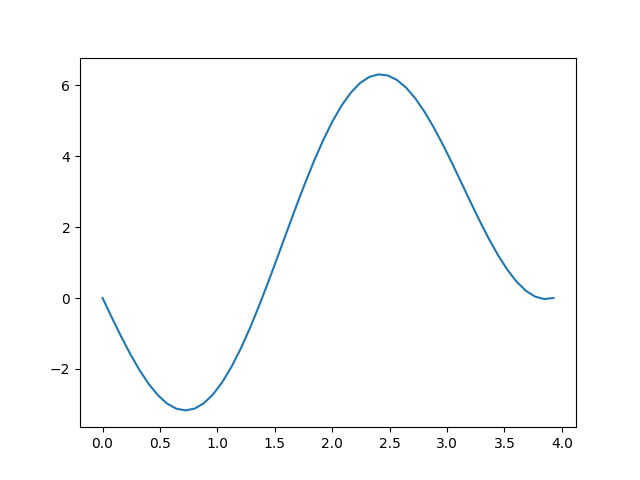
\includegraphics[width=5cm]{courbe.png}
\end{center}
 \end{frame}
 
 \begin{frame}[fragile] 
\begin{minted}[
mathescape,
framesep=2mm,
baselinestretch=1.2,
%fontsize=\footnotesize,
bgcolor=LightGray,
%linenos
]{python}
import numpy as np
import matplotlib.pyplot as plt
a = 0; b = 5 * np.pi / 4; t = np.linspace(a, b, 50)
y = t - 5 * np.pi / 4 * np.sin(2 * t)
plt.plot(t, y)
N = 10; h = (b - a) / (N + 1)
x = np.linspace(a, b, N + 2)
M = ((-2 + 4 * h ** 2) * np.diag(np.ones(N))
     + np.diag(np.ones(N - 1), -1)
     + np.diag(np.ones(N - 1), 1)) / (4*h**3)
F = np.arange(1,N+1,1)
U = np.linalg.solve(M, F)
U = np.insert(U, N, 0)
U = np.insert(U, 0, 0)
plt.plot(x, U)
plt.show()
\end{minted}
 
 \end{frame}
 
 \begin{frame} 
  \begin{center}
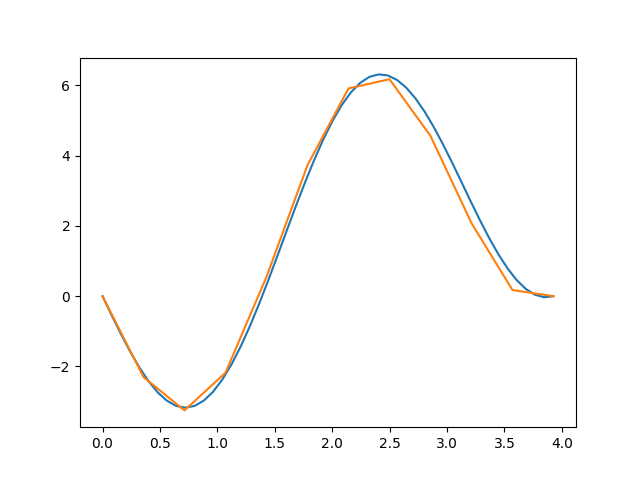
\includegraphics[width=10cm]{courbe2.png}
\end{center}
 \end{frame}
 
 
\begin{frame} 
La matrice $A_h$ est tridiagonale, on le décompose en deux matrices: 
\[A_h=\frac{1}{h^2} A_h^{(0)}+C_h\]

\[A_h^{(0)}=
\left(\begin{array}{ccccc}
2&-1&0&\cdots&0\\
-1&2&-1&\ddots&\vdots\\
0&  \ddots &\ddots&\ddots&0\\
\vdots &\ddots &-1&2&-1\\
   0&\cdots &0&-1 &2
\end{array}\right)
\] 
et
\[C_h=
\left(\begin{array}{cccc}
c_1&0&\cdots&0\\
0&c_2&\ddots&\vdots\\
  \vdots &\ddots&\ddots&0\\
   0&\cdots &0&c_n
\end{array}\right)
\]
On note que  les conditions au bord $u_0 = g_0$ et $u_{n+1} = g_1 $ n'apparaissent que dans le vecteur $b_h$.

  \end{frame}
  
 \begin{frame} 
 \begin{block}{proposition}
 Supposons $c \geqslant 0$. La matrice $A_h$ est symétrique définie positive.
 \end{block}


Démonstration La matrice $A_h$ est clairement symétrique. Soit z un vecteur de $\mathbb{R}^n$, de composantes $z_1,\cdots ,z_n$. On a
\[\begin{array}{ll}
z^t A_h z & = z^t A_h^{(0)} z  +\sum_{i=1}^nc_i z_i^2 \geqslant z^t A_h^{(0)} z\\
                & = \frac{z_1^2+(z_1-z_2)^2+\cdots +(z_{n-1}-z_n)^2+z_n^2}{h^2} 
\end{array} \]


Cette quantité est positive, et non nulle si $z \neq 0$ (car au moins l'un des termes au numérateur est non nul).

  \end{frame} 
  
  \begin{frame}
\begin{block}{Définition}
\[A_h^{(0)}=
\left(\begin{array}{ccccc}
2&-1&0&\cdots&0\\
-1&2&-1&\ddots&\vdots\\
0&  \ddots &\ddots&\ddots&0\\
\vdots &\ddots &-1&2&-1\\
   0&\cdots &0&-1 &2
\end{array}\right)
\] 

est la matrice du Laplacien discret.
\end{block}
\begin{block}{Théorème (Principe du maximum discret)}
$A_h V_h =F_h$ admet une solution unique $V_h$ de plus si $f\geq 0$ alors $V_h\geq 0$
\end{block}



\end{frame}

 \begin{frame}

\begin{block}{Lemme}
\[\forall V \in \mathbb{R}^n\qquad AV\geq 0 \Longrightarrow V\geq 0\]
\end{block}
\[  AV\geq 0 \Longrightarrow
 \left\{
 \begin{array}{l}
2V_1-V_2\geq 0\\
-V_{j-1}+2V_j-V_{j+1}\geq 0\\
-V_{n-1}+2V_n\geq 0
\end{array}
\right.
 \]
Soit $V_m=\inf_i(V_i)$
\begin{itemize}
\item $m=1$ : $2V_1-V_2\geq 0 \Longrightarrow V_1\geq V_2-V_1\geq 0 $
\item $m=n$ : $-V_{n-1}+2V_n \geq 0 \Longrightarrow V_n\geq V_{n-1}-V_n\geq 0 $
\item $m\neq n$ et $m \neq 1$ : 
\[-V_{m-1}+2V_m-V_{m+1}\geq 0  \Longrightarrow (V_m-V_{m+1})\geq (V_{m-1}-V_m)\geq 0\]
\[ \Longrightarrow V_m=V_{m+1}=V_{m-1} \Longrightarrow V_{m-1}=\inf_i(V_i)\Longrightarrow V_1=\inf_i(V_i)\]
\end{itemize}


\end{frame}

\begin{frame}
  \frametitle{Démo}
  \[AV=0 \Longrightarrow AV\geq 0 \mbox { et } AV\leq 0\Longrightarrow V\geq 0 \mbox { et } V\leq 0\Longrightarrow V=0\]
  Les coefficients de $A$ sont tous positifs: si $A^{-1}=[C_1\,C_2\,\cdots\,C_n]$ alors
  \[ A A^{-1}=I  \Longrightarrow A C_i =e_i \Longrightarrow C_i\geq 0 \Longrightarrow  A^{-1}\geq 0 \]
  $\Longrightarrow V = A^{-1}F\geq 0$
  
  
 \end{frame} 
  
  \begin{frame}
  \frametitle{Consistance}
  \begin{block}{Définition}
  Supposons $f\in C^2([0,1])$, donc $u\in C^4([0,1])$. On pose
  \[\begin{array}{ccc}
   \Pi_h:C^0([0,1])&\to &\mathbb{R}^n\\
  \omega&\mapsto &(\omega(x_1),\omega(x_2),\cdots,\omega(x_N))^T
  \end{array}\]
  On définit l'erreur de consistance par
  \[\varepsilon_h=A_h\Pi_h u-F_h\]
  On dit que le schéma est consistant si \[\lim_{n\to\infty}\|\varepsilon_h\|_{\infty}=0\]
  
  Si \[\|\varepsilon_h\|_{\infty} = O(h^p)\] On dit que la méthode est d'ordre $p$.
  \end{block}
  
 \end{frame} 

 \begin{frame}
  \frametitle{Consistance}
  \begin{block}{Proposition}
  Le schéma $A_h V_h =F_h$  est consistant d'ordre 2.
  \end{block}
  \[\begin{array}{lll}
  (\varepsilon_h)_j&=&\displaystyle  \frac{u(x_{j-1})-2u(x_j)+u(x_{j+1})}{h^2}-f(x_j)\\
  &=&\displaystyle   \frac{u(x_{j-1})-2u(x_j)+u(x_{j+1})}{h^2}-u''(x_j)=O(h^2)\\
  \end{array}\]
  \[\left|u(x_j+h)-u(x_j)-hu'(x_j)-\frac{h^2}{2}u''(x_j)-\frac{h^3}{6}u'''(x_j)\right|\leq \frac{h^4}{24}\|u^{(4)}\|_{\infty}\]
  \[- \frac{h^4}{24}\|u^{(4)}\|_{\infty}\leq u(x_j+h)-u(x_j)-hu'(x_j)-\frac{h^2}{2}u''(x_j)-\frac{h^3}{6}u'''(x_j)\leq \frac{h^4}{24}\|u^{(4)}\|_{\infty}\]
   \[- \frac{h^4}{24}\|u^{(4)}\|_{\infty}\leq u(x_j-h)-u(x_j)+hu'(x_j)-\frac{h^2}{2}u''(x_j)+\frac{h^3}{6}u'''(x_j)\leq \frac{h^4}{24}\|u^{(4)}\|_{\infty}\]
 \[\Longrightarrow \|\varepsilon_h\|_{\infty} \leq \frac{h^2}{12} \|u^{(4)}\|_{\infty}\] 
 
 \end{frame} 

 
 \begin{frame}
  \frametitle{Stabilité}
  \begin{block}{Définition}
  On dit que le schéma numérique $A_h V_h =F_h$  est stable s'il existe une constante $C$ telle que
  \[\|V_h\|\leq C\|F_h\|  \qquad \forall F_h\]
  \end{block}
  \begin{block}{Théorème}
   \[\|A_h^{-1}\|\leq \frac{1}{8}  \qquad \forall n\geq 1\]
  \end{block}
   Soit le problème 
   $\left\{\begin{array}{l}
   -u''=1\\
   u(0)=u(1)=0
   \end{array}\right.$ dont la solution est $u(x)=\frac{x(1-x)}{2}$
   Alors 
   \[F_h=\left(\begin{array}{c}1\\1\\ \vdots \\1 \end{array}\right)\Longrightarrow A_h^{-1}F_h = 
   \left(\begin{array}{c}\frac{h(1-h)}{2}\\\frac{2h(1-2h)}{2}\\ \vdots\\ \frac{nh(1-nh)}{2} \end{array}\right)
   \]
  \end{frame} 
 
 \begin{frame} 
   
   
 Donc \[ \|A_h^{-1}\|=\sup_{\|F_h\|=1}\|A_h^{-1}F_h\|=\frac 18\]
 \begin{block}{Définition}
  Soit $E_h=V_h-\Pi_h u$  On dit que le schéma numérique $A_h V_h =F_h$  converge  si pour tout $f\in C^0([0,1])$ 
  \[\|E_h\|_{\infty}\to 0 \quad \mbox{quand} n\to \infty\]
  \end{block}
 \begin{block}{Théorème}
  La méthode converge à l'ordre 2.
  \end{block}
  Démo: On note $u$ la solution exacte
  \[
  \begin{array}{ccl}
  A_hE_h&=& A_hV_h-A_h\Pi_h u\\
  &=& F_h-(\varepsilon_h+F_h)\\
  &=&-\varepsilon_h
  \end{array}
  \]
  \[\mbox{Donc } E_h=-A_h^{-1}\varepsilon_h\Longrightarrow \|E_h\|\leq \|A_h^{-1}\| \|\varepsilon_h\|\leq \frac{1}{8}\times \frac{h^2}{24} \|u^{(4)}\|\to 0 \]
 \end{frame} 
 


  \begin{frame} 
  \frametitle{Convergence de la méthode}
Afin d'étudier la convergence de la solution approchée $u_h$ vers la solution exacte $u$ lorsque $h \to 0$, on commence par étudier l'erreur de consistance :
 \begin{block}{definition}
On appelle erreur de consistance du schéma  $A_h u_h = b_h$, le vecteur $\epsilon_h(u)$ de $\mathbb{R}^n$ défini par
\[\epsilon_h(u) = A_h(\pi_h(u)) - b_h, \qquad \mbox{ où } 
\pi_h= \left(\begin{array}{c}
u(x_1)\\u(x_2)\\ \vdots \\ u(x_{n}) 
\end{array}\right)\]

$\pi_h(u)$ représente la projection de la solution exacte sur le maillage. On dit que le schéma est consistant pour la norme $\|\cdot \|$ de $\mathbb{R}^n$ si $\lim\limits_{h\to 0} \|\epsilon_h(u) \| = 0$. Si de plus il existe $C$ indépendante de $h$ telle que
\[\|\epsilon_h(u) \| \leqslant  C h^p\]
pour $p>0$, on dit que le schéma est d'ordre $p$ pour la norme $\|\cdot \|$ .
\end{block}

  \end{frame} 
   \begin{frame} 
 En utilisant (3), on obtient immédiatement
 
\[    \| \epsilon_h(u)  \|_{\infty}  \leq  \frac{h^2}{12} \sup_{y\in[0,1]} |u^{(4)}(y)|, \]

 et donc
 \begin{block}{proposition}
 Supposons que la solution $u$ du problème (1) est $C^4$  sur $[0, 1]$. Alors le schéma (4) est consistant d'ordre 2 pour la norme $\|\cdot \|_{\infty}$ .
 \end{block}


L'erreur de convergence est l'erreur entre la solution approchée $u_h$ est la solution exacte aux points du maillage $\pi_h(u)$. Afin de majorer cette erreur, il suffit d'observer que, par définition de l'erreur de consistance et puisque $A_h u_h = b_h$,

\[u_h - \pi_h(u) = -(A_h){-1}\epsilon_h(u).\]
On peut montrer que $\|(A_h)^{-1}\|\leq \frac{1}{8}$ (admis), ce qui donne le résultat de convergence :

    \end{frame} 
   \begin{frame} 
   \begin{theorem}
 On suppose $c \geqslant 0$. Si la solution $u$ du problème (1) est $C^4$ sur $[0, 1]$, alors le schéma (4) est convergent d'ordre 2 pour la norme $\|\cdot \|_{\infty}$. Plus précisément,
\[\|u_h -\pi_h(u)\|_{\infty} \leqslant \frac{h^2}{96}  \sup_{y\in[0,1]} |u^{(4)}(y)|.\]
 \end{theorem}
 
 
 
On notera que, dans cet exemple, la consistance du schéma permet immédiatement d'obtenir la convergence. Ceci est particulier à cet exemple simple. En général, un autre ingrédient est nécessaire à la convergence : la stabilité du schéma (voir section 2.3).


\end{frame}

\begin{frame}
\frametitle{Le problème aux limites d'ordre 2 en dimension 2}
Equation de Poisson $-\Delta u =f$
On considère le problème aux limites
\begin{equation}
\myredbox{\left\{\begin{array}{l}
{\displaystyle -\frac{\partial ^2 u}{\partial  x^2}-\frac{\partial ^2 u}{\partial  y^2} }=f(x,y), \quad(x,y)\in \Omega\\
u(x,y)=0,\quad (x,y)\in \partial\Omega
\end{array}\right.}
\end{equation}
 
où $f$ est une  fonction donnée sur $\Omega = [0, 1]\times [0, 1]$.
Les deux ingrédients principaux d'une approximation par différences finies sont le schéma d'approximation des dérivées et la grille de discrétisation.
 \end{frame}
 
  \begin{frame}
\frametitle{Approximation  par différences finies}
 \begin{center}
 \begin{tikzpicture}[domain=0:5]
  \draw[->] (-0.1,0) -- (5.5,0)  node[right] {$\scriptstyle x$};
  \draw[->] (0,-0.1) -- (0,5.2) node[above] {$\scriptstyle y$};
  \path[fill=black]  (0,0) circle (.4mm) [fill=orange] node[below] {$\scriptstyle 0=x_0$};
 \path[fill=black]  (1,0) circle (.4mm) [fill=orange];
  \path[fill=black]  (2,0) circle (.4mm) [fill=orange] node[below] {$\scriptstyle x_{i-1}$};
  \path[fill=black]  (3,0) circle (.4mm) [fill=orange] node[below] {$\scriptstyle x_{i}$};
 \path[fill=black]  (4,0) circle (.4mm) [fill=orange] node[below] {$\scriptstyle x_{i+1}$};
   \draw  (1.5,0.5) node {$\scriptstyle h_x$};
   \draw[<->] (1,0.2) -- ++(1,0) ;
   \path[fill=black]  (5,0) circle (.4mm) [fill=orange] node[below] {$\scriptstyle 1$};

 %\path[fill=black]  (0,0) circle (.4mm) [fill=orange] node[below] {$\scriptstyle 0=x_0$};
 \path[fill=black]  (0,1) circle (.4mm) [fill=orange];
  \path[fill=black]  (0,2) circle (.4mm) [fill=orange] node[left] {$\scriptstyle y_{i-1}$};
  \path[fill=black]  (0,3) circle (.4mm) [fill=orange] node[left] {$\scriptstyle y_{i}$};
 \path[fill=black]  (0,4) circle (.4mm) [fill=orange] node[left] {$\scriptstyle y_{i+1}$};
   \draw  (1.5,0.5) node {$\scriptstyle h_x$};
   \draw[<->] (1,0.2) -- ++(1,0) ;
    \draw[<->] (0.2,1) -- ++(0,1) ;
     \draw  (0.5,1.5) node {$\scriptstyle h_y$};
   \path[fill=black]  (0,5) circle (.4mm) [fill=orange] node[left] {$\scriptstyle 1$};
\draw[dotted,blue] (2,0) -- ++(0,5) ;
\draw[dotted,blue] (3,0) -- ++(0,5) ;
\draw[dotted,blue] (4,0) -- ++(0,5) ;
\draw[dotted,blue] (0,2) -- ++(5,0) ;
\draw[dotted,blue] (0,3) -- ++(5,0) ;
\draw[dotted,blue] (0,4) -- ++(5,0) ;
 \path[fill=black]  (3,3) circle (.5mm) [fill=red] node[above right] {$\scriptstyle u_{i,j}$};
 \path[fill=black]  (2,3) circle (.5mm) [fill=red] node[above right] {$\scriptstyle u_{i-1,j}$};
 \path[fill=black]  (4,3) circle (.5mm) [fill=red] node[above right] {$\scriptstyle u_{i+1,j}$};
 \path[fill=black]  (3,2) circle (.5mm) [fill=red] node[above right] {$\scriptstyle u_{i,j-1}$};
 \path[fill=black]  (3,4) circle (.5mm) [fill=red] node[above right] {$\scriptstyle u_{i,j+1}$};

\end{tikzpicture}
 \end{center}
Les points de discrétisation du maillage : $M_{i,j}=(x_i,y_j)=(ih_x,j h_y)$
\[(i ,j) \in \llbracket 0,N_x+1\rrbracket \times \llbracket 0,N_y+1\rrbracket,\quad h_x=\frac{1}{N_x+1}, h_y=\frac{1}{N_y+1} \]
\end{frame}
 
 
 \begin{frame}
Les points 
\[\left\{\begin{array}{l}
M_{0,j} \mbox{ et } M_{N_x+1,j}\mbox{ pour } j=0,1,\cdots,N_y+1\\
M_{i,0} \mbox{ et } M_{i,N_y+1}\mbox{ pour } i=0,1,\cdots,N_x+1
\end{array}\right.\]
constituent le bord du domaine (les cotés du rectangle  $OABC$), et les points $M_{i,j}$ où $(i,j)\in  \llbracket 1,N_x\rrbracket \times \llbracket 1,N_y\rrbracket $ sont les points internes du maillage.

 \begin{center}
 \begin{tikzpicture}[domain=0:5,scale=0.7]
  \draw[->] (-0.1,0) -- (5.5,0)  node[right] {$\scriptstyle x$};
  \draw[->] (0,-0.1) -- (0,5.3) node[above] {$\scriptstyle y$};
  \path[fill=black]  (0,0) circle (.4mm) [fill=orange] node[below] {$\scriptstyle O$};


   \path[fill=black]  (5,0) circle (.4mm) [fill=orange] node[below] {$\scriptstyle A$};

   \path[fill=black]  (0,5) circle (.4mm) [fill=orange] node[left] {$\scriptstyle C$};
      \path[fill=black]  (5,5) circle (.4mm) [fill=orange] node[above right] {$\scriptstyle B$};
\draw[dotted,blue] (2,0) -- ++(0,5) ;
\draw[dotted,blue] (3,0) -- ++(0,5) ;
\draw[dotted,blue] (4,0) -- ++(0,5) ;
\draw[dotted,blue] (0,2) -- ++(5,0) ;
\draw[dotted,blue] (0,3) -- ++(5,0) ;
\draw[dotted,blue] (0,4) -- ++(5,0) ;
\draw[orange] (0.02,0.02) -- ++(5,0)  -- ++(0,5) -- ++(-5,0)  -- ++(0,-5)  ;
 \path[fill=red]  (3,3) circle (.8mm)node[above right] {$\scriptstyle u_{i,j}$};
 \path[fill=blue]  (3,0) circle (.8mm) node[below] {$\scriptstyle u_{i,0}$};
 \path[fill=blue]  (5,3) circle (.8mm)node[right] {$\scriptstyle u_{N_x+1,j}$};
  \path[fill=blue]  (3,5) circle (.8mm) node[above] {$\scriptstyle u_{i,N_y+1}$};
  \path[fill=blue]  (0,3) circle (.8mm)  node[ left] {$\scriptstyle u_{0,j}$};
  
\end{tikzpicture}
 \end{center}

On cherche en chaque point $M_{i,j}$ une valeur approchée $u_{i,j}\simeq u(x_i,y_j)$. 

Les valeurs  $u_{i,j}$ sur les bord sont nulles (ou données par hypothèse).
\end{frame}
 
 
 \begin{frame}

 Pour les sommets internes, on utilise l'approximation  de la dérivée seconde décrite plus haut. On a
\begin{equation}
\myredbox{\left\{\begin{array}{l}
{\displaystyle -\frac{\partial ^2 u(x_i,y_j)}{\partial  x^2}-\frac{\partial ^2 u(x_i,y_j)}{\partial  y^2} }=f(x_i,y_j), \quad (x_i,y_j)\in  ]0,1[  \times ]0,1[\\
u(x_i,0)=u(x_i,1)=0,\quad 0\leq x_i\leq 1\\
u(0,y_j)=u(1,y_j)=0,\quad 0\leq y_j \leq 1
\end{array}\right.}
\end{equation}
Or
\[\frac{\partial ^2 u(x_i,y_j)}{\partial  x^2}\simeq \frac{u(x_i-h,y_j)-2u(x_i,y_j)+u(x_i+h,y_j)}{h_x^2}\simeq \frac{u_{i-1,j}-2u_{i,j}+u_{i+1,j}}{h_x^2}\] 
\[\frac{\partial ^2 u(x_i,y_j)}{\partial  y^2}\simeq \frac{u(x_i,y_j-h)-2u(x_i,y_j)+u(x_i,y_j+h)}{h_y^2}\simeq \frac{u_{i,j-1}-2u_{i,j}+u_{i,j+1}}{h_y^2}\] 
 
 et on pose où $f_{i,j}=f(x_i,y_j)$.
 \end{frame}
 
 
 \begin{frame}
D'où le schéma, pour $i\in  \llbracket 0,N_x+1\rrbracket$ et $j\in  \llbracket 0,N_y+1\rrbracket$:
\begin{equation}
\myredbox{\left\{\begin{array}{l}
\mbox{ Pour } (i,j)\in  \llbracket 1,N_x\rrbracket \times \llbracket 1,N_y\rrbracket\\
{\displaystyle -\frac{u_{i-1,j}-2u_{i,j}+u_{i+1,j}}{h_x^2}-\frac{u_{i,j-1}-2u_{i,j}+u_{i,j+1}}{h_y^2} }=f_{i,j} \\
\mbox{ et } \\
u_{i,0}=u_{i,N_y+1}=0,\quad i\in  \llbracket 0,N_x+1\rrbracket\\
u_{0,j}=u_{N_x+1,j}=0,\quad j\in  \llbracket 0,N_y+1\rrbracket
\end{array}\right.}
\end{equation}
On obtient $N_x\times N_y$ équations à $N_x\times N_y$ inconnues 
\[u_{1,1}; u_{1,2}; \cdots , u_{1,N_y}; u_{2,1}; u_{2,2} \cdots  u_{2,N_y} \cdots    \cdots    u_{N_x,1};u_{N_x,2} \cdots  u_{N_x,N_y}\]
 \end{frame}
 
\begin{frame} 


\[\begin{array}{l}
i=1, j=1:\quad {\displaystyle -\frac{u_{0,1}-2u_{1,1}+u_{2,1}}{h_x^2}-\frac{u_{1,0}-2u_{1,1}+u_{1,2}}{h_y^2} }=f_{1,1} \\
i=1, j=2:\quad {\displaystyle -\frac{u_{0,2}-2u_{1,2}+u_{2,2}}{h_x^2}-\frac{u_{1,1}-2u_{1,2}+u_{1,3}}{h_y^2} }=f_{1,2} \\
\cdots\\
i=1, j=N_y:\quad {\displaystyle -\frac{u_{0,N_y}-2u_{1,N_y}+u_{2,N_y}}{h_x^2}-\frac{u_{1,N_y-1}-2u_{1,N_y}+u_{1,N_y+1}}{h_y^2} }=f_{1,2} \\
i=2, j=1:\quad {\displaystyle -\frac{u_{1,1}-2u_{2,1}+u_{3,1}}{h_x^2}-\frac{u_{2,0}-2u_{2,1}+u_{2,2}}{h_y^2} }=f_{2,1} \\
i=2, j=2:\quad {\displaystyle -\frac{u_{1,2}-2u_{2,2}+u_{3,2}}{h_x^2}-\frac{u_{2,1}-2u_{2,2}+u_{2,3}}{h_y^2} }=f_{2,2} \\
\cdots\\
i=2, j=N_y:\quad {\displaystyle -\frac{u_{1,N_y}-2u_{2,N_y}+u_{3,N_y}}{h_x^2}-\frac{u_{2,N_y-1}-2u_{2,N_y}+u_{2,N_y+1}}{h_y^2} }=f_{1,2} \\
%i=N_x, j=1:\quad {\displaystyle -\frac{u_{N_x-1,1}-2u_{N_x,1}+u_{N_x+1,1}}{h_x^2}-\frac{u_{N_x,0}-2u_{N_x,1}+u_{N_x,2}}{h_y^2} }=f_{N_x,1} \\
%i=N_x, j=2:\quad {\displaystyle -\frac{u_{N_x-1,2}-2u_{N_x,2}+u_{N_x+1,2}}{h_x^2}-\frac{u_{N_x,1}-2u_{N_x,2}+u_{N_x,3}}{h_y^2} }=f_{N_x,2} \\
\cdots\\
i=N_x, j=N_y:\quad {\displaystyle -\frac{u_{N_x-1,N_y}-2u_{N_x,N_y}+u_{N_x+1,N_y}}{h_x^2}-\frac{u_{N_x,N_y-1}-2u_{N_x,N_y}+u_{N_x,N_y+1}}{h_y^2} }=f_{N_x,N_y} 
\end{array}
\]

 \end{frame}
 
\begin{frame} 
D'où le système, en faisant $N_x=N_y=n$ et donc $h_x=h_y=h$:
\[\left\{\begin{array}{l}
4u_{1,1}-u_{1,2}-u_{2,1}=h^2f_{1,1}\\
   -u_{1,1}+4u_{1,2}-u_{1,3} -u_{2,2} =h^2f_{1,2}\\
   \cdots\\
  -u_{1,n-1}+4u_{1,n} -u_{2,n} =h^2f_{1,n}\\
\hline
   -u_{1,1}+4u_{2,1}-u_{2,2}-u_{3,1}  =h^2f_{2,1}\\
   -u_{1,2}+4u_{2,2}-u_{2,3}-u_{3,2}  =h^2f_{2,2}\\
     \cdots\\
     -u_{1,n}-u_{2,n-1}+4u_{2,n} -u_{3,n} =h^2f_{2,n}\\
  \hline
      \vdots\\
      \hline  
     -u_{n-1,1}+4u_{n,1}-u_{n,2}  =h^2f_{n,1}\\
   -u_{n-1,2}+4u_{n,2}-u_{n,3} =h^2f_{n,2}\\
     \cdots\\
     -u_{n-1,n}-u_{n,n-1}+4u_{n,n}  =h^2f_{n,n}\\    
\end{array}\right.
\]


 \end{frame}
 
\begin{frame} 

 Matriciellement, le problème s'écrit : 
 
 \begin{equation}
 \myredbox{A_h u_h =b_h}
 \end{equation}
 
  avec
 

 
 \[
\left[\begin{array}{cccc|cccc|cccc|cccc}
4&-1&0&0&-1&0&0&0\\
-1&4&-1&0&0&-1&0&0\\
0&-1&4&-1&0&0&-1&0\\
0&0&-1&4&0&0&0&-1 \\ \hline
-1&0&0&0&4&-1&0&0&-1&0&0&0\\
0&-1&0&0&-1&4&-1&0&0&-1&0&0\\
0&0&-1&0&0&-1&4&-1&0&0&-1&0\\
0&0&0&-1&0&0&-1&4&0&0&0&-1\\ \hline
&&&&-1&0&0&0&4&-1&0&0&-1\\
&&&&0&-1&0&0&-1&4&-1&0&0&-1\\
&&&&0&0&-1&0&0&-1&4&-1&0&0&-1\\
&&&&0&0&0&-1&0&0&-1&4&0&0&0&-1\\ \hline
&&&&&&&&-1&0&0&0&4&-1\\
&&&&&&&&0&-1&0&0&-1&4&-1\\
&&&&&&&&0&0&-1&0&0&-1&4&-1\\
&&&&&&&&0&0&0&-1&0&0&-1&4
\end{array}\right]
\] 
 

\[u_h =\left(\begin{array}{c}
u_1\\u_2\\ \vdots \\ u_{n-1} \\ u_n
\end{array}\right), \qquad b_h =\left(\begin{array}{c}
f_1+\frac{g_0}{h^2}\\f_2\\ \vdots \\ f_{n-1} \\ f_n+\frac{g_1}{h^2}
\end{array}\right)
\]

\end{frame}
 
 \begin{frame}  
 \[
\left[\begin{array}{ccc|ccc|ccc}
4&-1&0&-1&0&0\\
-1&4&-1&0&-1&0\\
0&-1&4&0&0&-1\\  \hline
-1&&&4&-1&0&-1&0&0\\
&-1&&-1&4&-1&0&-1&0\\
&&-1&0&-1&4&0&0&-1\\  \hline
&&&-1&&&4&-1&0\\
&&&&-1&&-1&4&-1\\
&&&&&-1&0&-1&4
\end{array}\right]
\left[\begin{array}{c}
u_{11}\\u_{12}\\ u_{13} \\  \hline
u_{21}\\u_{22}\\ u_{23} \\  \hline
u_{31}\\u_{32}\\ u_{33}
\end{array}\right] =h^2\left[\begin{array}{c}
f_{11}\\f_{12}\\ f_{13} \\ \hline
 f_{21}\\f_{22}\\ f_{23} \\  \hline
 f_{31}\\f_{32}\\ f_{33}
\end{array}\right]
\] 
 
\end{frame}

\begin{frame}
 \begin{center}
 \begin{tikzpicture}[domain=0:5]
  \draw[->] (-0.1,0) -- (4.5,0)  node[right] {$\scriptstyle x$};
  \draw[->] (0,-0.1) -- (0,4.3) node[above] {$\scriptstyle y$};
  \path[fill=black]  (0,0) circle (.4mm) [fill=orange] node[below] {$\scriptstyle O$};


   \path[fill=black]  (4,0) circle (.4mm) [fill=orange] node[below] {$\scriptstyle A$};

   \path[fill=black]  (0,4) circle (.4mm) [fill=orange] node[left] {$\scriptstyle C$};
      \path[fill=black]  (4,4) circle (.4mm) [fill=orange] node[above right] {$\scriptstyle B$};
\draw[dotted,blue] (1,0) -- ++(0,4) ;
\draw[dotted,blue] (2,0) -- ++(0,4) ;
\draw[dotted,blue] (3,0) -- ++(0,4) ;
\draw[dotted,blue] (0,1) -- ++(4,0) ;
\draw[dotted,blue] (0,2) -- ++(4,0) ;
\draw[dotted,blue] (0,3) -- ++(4,0) ;
\draw[orange] (0.02,0.02) -- ++(4,0)  -- ++(0,4) -- ++(-4,0)  -- ++(0,-4)  ;
 \path[fill=red]  (1,1) circle (.5mm)node[below] {$\scriptstyle 0$};
 \path[fill=red]  (2,1) circle (.5mm) node[below] {$\scriptstyle 1$};
 \path[fill=red]  (3,1) circle (.5mm)node[below] {$\scriptstyle 2$};
  \path[fill=red]  (1,2) circle (.5mm) node[below] {$\scriptstyle 3$};
  \path[fill=red]  (2,2) circle (.5mm)  node[ below] {$\scriptstyle 4$};
   \path[fill=red]  (3,2) circle (.5mm)  node[ below] {$\scriptstyle 5$};
   \path[fill=red]  (1,3) circle (.5mm) node[below] {$\scriptstyle 6$};
  \path[fill=red]  (2,3) circle (.5mm)  node[ below] {$\scriptstyle 7$};
   \path[fill=red]  (3,3) circle (.5mm)  node[ below] {$\scriptstyle 8$};
  
\end{tikzpicture}
\[(i,j)\mapsto (j-1)N+i-1 \]
 \end{center}
\end{frame}

\begin{frame}[fragile] 
\begin{minted}[
mathescape,
framesep=2mm,
baselinestretch=1.2,
%fontsize=\footnotesize,
bgcolor=LightGray,
%linenos
]{python}
import matplotlib.pyplot as plt
from matplotlib import cm
import numpy as np
N = 3; h = 1 / (N + 1)
# La matrice
M = np.diag(4 * np.ones(N * N)) \
    - np.diag(np.ones(N * N - 1), -1) \
    - np.diag(np.ones(N * N - 1), 1) \
    - np.diag(np.ones(N * N - N), -N) \
    - np.diag(np.ones(N * N - N), N)
for k in range(N - 1):
    M[(k + 1) * N, (k + 1) * N - 1] = 0
    M[(k + 1) * N - 1, (k + 1) * N] = 0
F = h * h * np.ones(N * N)
U = np.linalg.solve(M, F)
\end{minted}
 

 \end{frame}


\begin{frame}[fragile] 
\begin{minted}[
mathescape,
framesep=2mm,
baselinestretch=1.2,
%fontsize=\footnotesize,
bgcolor=LightGray,
%linenos
]{python}
fig = plt.figure()
ax = fig.add_subplot(projection = '3d') 
# Make data.
X = np.linspace(0, 1, N + 2)
Y = np.linspace(0, 1, N + 2)
X, Y = np.meshgrid(X, Y)
Z = np.zeros((N + 2, N + 2))
for i in range(1, N + 1):
    for j in range(1, N + 1):
        Z[i, j] = U[(i - 1) * N + j - 1]
# Plot the surface.
surf = ax.plot_surface(X, Y, Z, rstride=1, cstride=1,
     cmap=cm.coolwarm,linewidth=0, antialiased=False)
fig.colorbar(surf, shrink=0.5, aspect=10)
plt.show()
\end{minted}

\end{frame}

\begin{frame}
\frametitle{$N=3$}
 \begin{center}
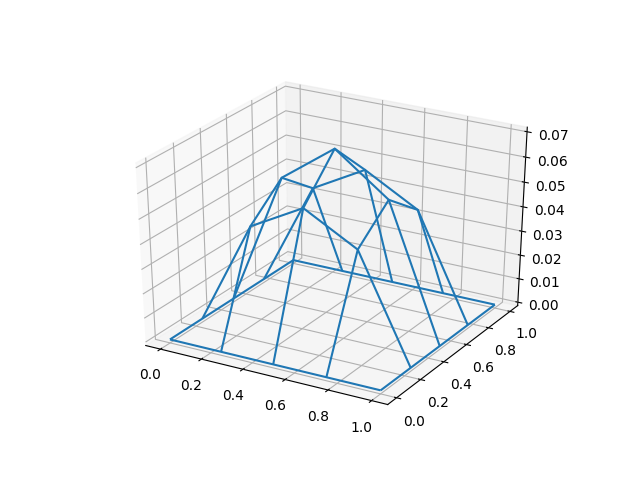
\includegraphics[width=7cm]{surface.png}
\end{center}
\end{frame}

\begin{frame}
\frametitle{$N=3$}
 \begin{center}
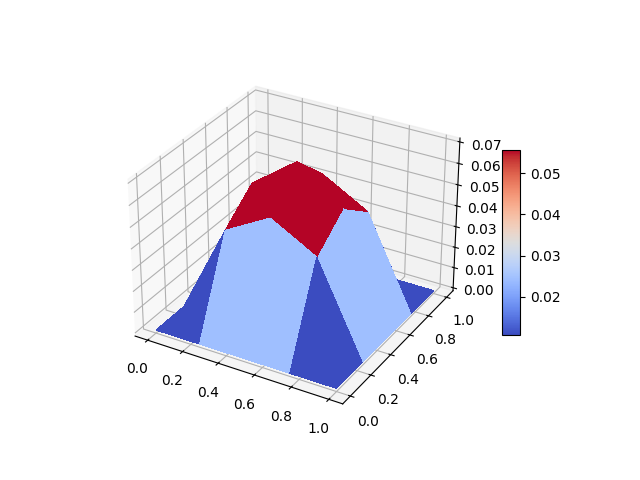
\includegraphics[width=12cm]{surfaceN3.png}
\end{center}
\end{frame}

\begin{frame}
\frametitle{$N=10$}
 \begin{center}
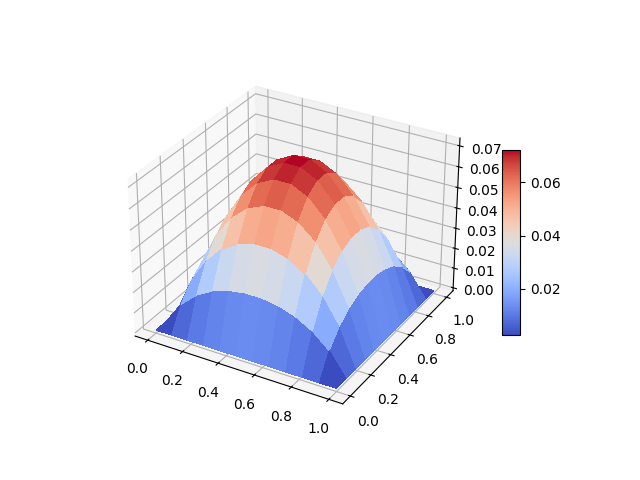
\includegraphics[width=12cm]{surfaceN10.png}
\end{center}
\end{frame}


\begin{frame}
\frametitle{$N=50$}
 \begin{center}
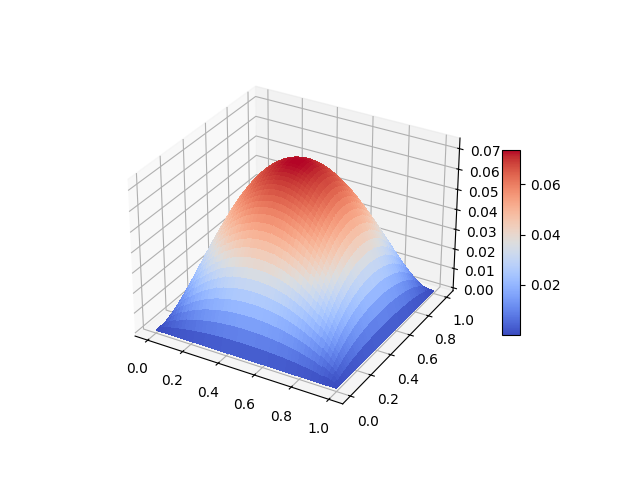
\includegraphics[width=12cm]{surfaceN50.png}
\end{center}
\end{frame}

\begin{frame}
\frametitle{$N=100$}
 \begin{center}
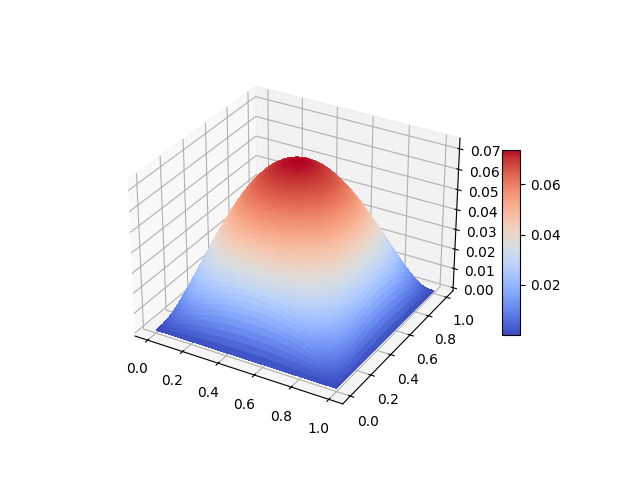
\includegraphics[width=12cm]{surfaceN100.png}
\end{center}
\end{frame}






















  \section{L’équation de la chaleur en dimension 1}
 \begin{frame}   
  \frametitle{les schémas implicites et explicites}
On s'intéresse au problème
\[\left\{\begin{array}{l}
\displaystyle \frac{\partial u}{\partial t}(t,x) - \frac{\partial^2 u}{\partial x^2}(t,x) = f(t,x), \mbox{ pour }(t,x)\in [0,T]\times  [0,1]\\
u(0,x)=u_0(x), \mbox{ pour } x\in [0,1]\\
u(t,0)=0 \mbox{ et }  u(t,1) = 0, \mbox{ pour } t\geqslant 0,
\end{array}\right.\]


où l'on a pris pour simplifier des conditions au bord nulles. Il s'agit de l'équation de la chaleur en dimension 1 (d'espace), qui est un problème parabolique en dimension 2 (temps et espace). Cet exemple est typique de la situation générale des problèmes paraboliques. On distingue deux grandes familles d'approximations par différences finies : les schémas explicites et les schémas implicites.
  \end{frame}
  
  
  \begin{frame}   
  \frametitle{La discétisation}
 On va se limiter au cas le plus simple du maillage régulier : soient $n$, $m$ deux entiers fixés. On pose
  \[x_i =i h,\quad \forall i\in\{0,1,...,n+1\},\quad \mbox{ où } h=\frac 1{n+1}\]
\[t_j =j \Delta t,\quad \forall j\in\{0,1,...,m\},\quad \mbox{ où } \Delta t= \frac{1}{m} .\]

  En particulier, $x_0 = 0$, $x_{n+1} = 1$, $t_0 = 0$ et $t_{m} = T$. Les points $(t_j,x_i)$
sont alors les points d'intersection d'une "grille" régulière en espace-temps.

L'approximation par différences finies consiste alors à chercher une approximation, notée $u_i^{(j)}$, de $u(t_j,x_i)$ (notez que l'indice en temps est en exposant, et l'indice en espace en indice, comme précédemment).

Les valeurs approchées aux points de maillage au bord du domaine et en $t = 0$ sont données par la valeur exacte ( donnée ) de la fonction $u$ :

\end{frame}
 
  \begin{frame}   
\begin{equation}
u_0^{(j)} =u_{n+1}^{(j)} =0,\quad \forall j\in\{0,...,m\} 
\end{equation}
\begin{equation}
u_i^{(0)} =u_{0}(x_i),\quad \forall j\in\{0,...,n+1\} 
\end{equation}

Ceci laisse $n m$  inconnues à déterminer ( les $u_i^{(j)}$ pour $1 \leqslant i \leqslant n$ et $1 \leqslant j \leqslant m)$. 

 On a déjà vu que le terme de dérivée seconde pouvait être approché avec


\[\frac{\partial^2 u}{\partial x^2}(x_i,t_j) \simeq \frac{u(x_{i+1},t_j)-2u(x_{i},t_j)+u(x_{i-1},t_j)}{h^2}\simeq
\frac{u_{i+1}^{(j)}-2u_{i}^{(j)}+u_{i-1}^{(j)}}{h^2}\]

   (schéma à trois points pour la dérivée seconde). Plusieurs choix sont possibles pour l'approximation de la dérivée en temps. Chacun de ces choix conduit à une famille de schémas distincte.
 \end{frame}
  
 


  \begin{frame}    
  \frametitle{Le schéma explicite}
La première possibilité est d'utiliser l'approximation décentrée à droite
\[\frac{\partial u}{\partial t}(x_i,t_j) \simeq \frac{u(x_{i},t_{j+1})-u(x_{i},t_j)}{\Delta t}\simeq
\frac{u_{i}^{(j+1)}-u_{i}^{(j)} }{\Delta t}\]


On obtient alors le schéma suivant :

\[
\frac{u_{i}^{(j+1)}-u_{i}^{(j)} }{\Delta t} - \frac{u_{i+1}^{(j)}-2u_{i}^{(j)}+u_{i-1}^{(j)}}{h^2} = f(x_i,t_j), \quad \forall i\in\{1,...,n\} ,  \forall j\in\{0,...,m\} 
\]


soit $n \times m$ équations pour $n \times m$  inconnues. On note que les conditions aux limites (8) et (9) doivent être connues pour résoudre ces équations, et que l'indice de temps $j$ doit varier entre $0$ et $m$.

   \end{frame}
   \begin{frame}    
Il est commode de réécrire ce système vectoriellement : on introduit la notation
\[U^{(j)} =\left(\begin{array}{c}
u_1^{(j)}\\u_2^{(j)}\\ \vdots \\  u_n^{(j)}
\end{array}\right),\quad \forall j\in\{0,...,m\} \]

Le vecteur $U^{(0)}$ est donné par les conditions initiales, et le schéma précédent s'écrit :

   \begin{equation}
   \frac{U^{(j+1)}-U^{(j)} }{\Delta t} +A_h^{(0)}U^{(j)} =C^{(j)} , \quad \forall j\in\{0,...,m\} 
   \end{equation}

où la matrice $A_h^{(0)}$ a été définie dans (6), et

\[C^{(j)} =\left(\begin{array}{c}
f(x_1,t^{(j)})\\f(x_2,t^{(j)})\\ \vdots \\  f(x_n,t^{(j)})
\end{array}\right),\quad \forall j\in\{0,...,m\} \]
     \end{frame}
  
\begin{frame}      
 Ce système peut également se réécrire sous la forme
   \begin{equation}
  U^{(j+1)}=(I_d - \Delta t A_h^{(0)})U^{(j)}  +\Delta tC^{(j)} , \quad \forall j\in\{0,...,m-1\} 
   \end{equation}

où on utilise la notation $I_d$ pour la matrice identité.

Cette équation justifie le nom explicite pour ce schéma, puisqu'il permet
de calculer la valeur approchée au temps $t_{j+1}$ par simple produit de matrice avec la valeur approchée au temps $t_{j}$ . En particulier, aucune inversion de matrice ou résolution de système linéaire n'est nécessaire pour le calcul.

 \end{frame} 
  

 \begin{frame}     
  \frametitle{Exemple}
  \begin{center}
 \begin{tikzpicture}[scale=0.8]
  \draw[->] (-0.1,0) -- (4.5,0)  node[right] {$\scriptstyle x$};
  \draw[->] (0,-0.1) -- (0,2.3) node[above] {$\scriptstyle \theta$};
  \path[fill=black]  (0,0) circle (.4mm) node[below] {$\scriptstyle O$};
 \path[fill=black]  (1,0) circle (.4mm)  ;
 \path[fill=black]  (2,0) circle (.4mm) ; 
  \path[fill=black]  (3,0) circle (.4mm) ;
   \path[fill=black]  (4,0) circle (.4mm)  node[below] {$\scriptstyle A$};
	\draw[<->] (1,-0.2) -- ++(1,0);
 \draw  (1.5,-0.5) node {$\scriptstyle h=\frac{1}{n+1}$};

%\draw[dotted,red] (0,2) -- ++(4,0) node[right] {$\scriptstyle \theta_0=100$°};
 \draw[color=blue][domain=0:4]   plot (\x,{2*sin(3.14/2*\x r)});
  \draw  (2.4,1.8) node[blue]{$\scriptstyle \theta_0=\sin (2\pi x)$};
\draw[fill=orange] (0.02,0.02) -- ++(4,0)  -- ++(0,0.04) -- ++(-4,0)  -- ++(0,-0.04)  ;
\end{tikzpicture}
 \end{center}
  \[\Delta t = 0.01\]
  \[\left\{\begin{array}{l}
  U^{(j+1)}=\left[ I_n -\frac{\Delta t}{h^2}\left( 
  \begin{array}{ccc}
  2&-1&0\\
  -1&2&-1\\
  0&-1&2\\
  \end{array}
  \right)\right]U^{(j)}\\
  U^{(0)}=\left( \begin{array}{c}
  100\\
  0\\
  -100\\
  \end{array}
  \right)
  
  \end{array}\right.
  \]
  
   \end{frame}
   
  \begin{frame}[fragile] 
\begin{minted}[
mathescape,
framesep=2mm,
baselinestretch=1.2,
%fontsize=\footnotesize,
bgcolor=LightGray,
%linenos
]{python}
import matplotlib.pyplot as plt
import numpy as np

N = 50;
M = 5;
h = 1 / (N + 1);
dt = 0.01
x = np.linspace(0, 1, N + 2)

# La matrice
A = np.diag(2 * np.ones(N)) \
    - np.diag(np.ones(N - 1), -1) \
    - np.diag(np.ones(N - 1), 1)

  \end{minted}

\end{frame}


 \begin{frame}[fragile] 
\begin{minted}[
mathescape,
framesep=2mm,
baselinestretch=1.2,
%fontsize=\footnotesize,
bgcolor=LightGray,
%linenos
]{python}

# Theta initiale
U = 100 * np.sin(2*np.pi*x)
plt.plot(x, U)
for k in range(1, M):
  U[1:-1] = np.dot((np.eye(N) - dt / (h ** 2) * A), U[1:-1])
  plt.plot(x, U)

plt.savefig('chaleurExplicite.png')
plt.show()
  \end{minted}

\end{frame}

\begin{frame}
 \begin{center}
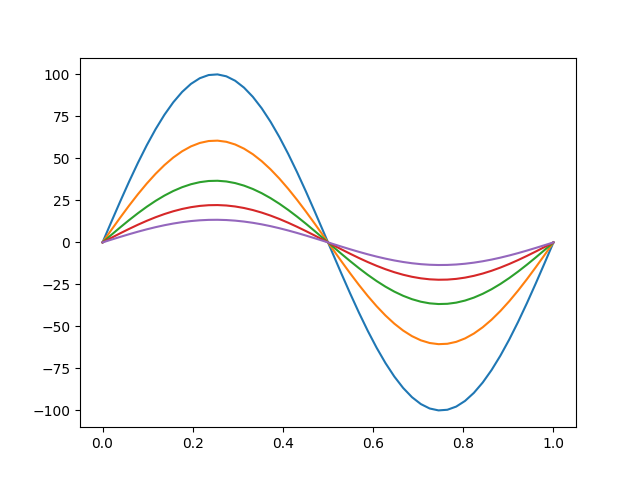
\includegraphics[width=7cm]{chaleurExplicite.png}
\end{center}
\end{frame}
  
  
  
\begin{frame}    
  \frametitle{Le schéma implicite}
On aurait pu approcher la dérivée partielle en temps par l'approximation décentrée à gauche
\[\frac{\partial u}{\partial t}(x_i,t_j) \simeq \frac{u(x_{i},t_{j})-u(x_{i},t_{j-1})}{\Delta t}\simeq
\frac{u_{i}^{(j)}-u_{i}^{(j-1)} }{\Delta t}\]


On obtient alors le schéma suivant :

\[
\frac{u_{i}^{(j)}-u_{i}^{(j-1)} }{\Delta t} - \frac{u_{i+1}^{(j)}-2u_{i}^{(j)}+u_{i-1}^{(j)}}{h^2} = f(x_i,t_j), \quad \forall i\in\{1,...,n\} ,  \forall j\in\{1,...,m\} 
\]

couplé aux mêmes conditions initiales que le schéma explicite (noter que cette fois l'indice $j$ varie de $1$ à $m$). Vectoriellement, on obtient
 \end{frame} 
  
\begin{frame}     
  \begin{equation}
   \frac{U^{(j)}-U^{(j-1)} }{\Delta t} +A_h^{(0)}U^{(j)} =C^{(j)} , \quad \forall j\in\{1,...,m\} 
   \end{equation}

où les $C^{(j)}$ sont définis comme plus haut, ce qui se réécrit

   \begin{equation}
  U^{(j)}=(I_d + \Delta t A_h^{(0)})^{-1}\left(U^{(j-1)}  +\Delta t C^{(j)} \right), \quad \forall j\in\{1,...,m\} 
   \end{equation}

 On remarque que la matrice $(I_d + \Delta t A_h^{(0)})$ est symétrique définie positive, et donc inversible, puisque $A_h^{(0)}$ est symétrique définie positive. 
 
Ce schéma est dit implicite puisque, contrairement au schéma explicite, sa résolution nécessite la résolution d'un système linéaire à chaque pas de temps (ou le calcul initial de l'inverse de la matrice $(I_d + \Delta t A_h^{(0)})$, utilisé ensuite à chaque pas de temps). La résolution du schéma implicite est donc plus coûteuse que le schéma explicite. Cependant, comme on le verra plus loin, ce coût en temps de calcul est largement compensé par la meilleure stabilité du schéma. 
  \end{frame}  
  
  \begin{frame}     
  \frametitle{Exemple}
   \begin{center}
 \begin{tikzpicture}[scale=0.8]
  \draw[->] (-0.1,0) -- (4.5,0)  node[right] {$\scriptstyle x$};
  \draw[->] (0,-0.1) -- (0,2.3) node[above] {$\scriptstyle \theta$};
  \path[fill=black]  (0,0) circle (.4mm) node[below] {$\scriptstyle O$};
 \path[fill=black]  (1,0) circle (.4mm)  ;
 \path[fill=black]  (2,0) circle (.4mm) ; 
  \path[fill=black]  (3,0) circle (.4mm) ;
   \path[fill=black]  (4,0) circle (.4mm)  node[below] {$\scriptstyle A$};
	\draw[<->] (1,-0.2) -- ++(1,0);
 \draw  (1.5,-0.5) node {$\scriptstyle h=\frac{1}{n+1}$};

%\draw[dotted,red] (0,2) -- ++(4,0) node[right] {$\scriptstyle \theta_0=100$°};
 \draw[color=blue][domain=0:4]   plot (\x,{2*sin(3.14/2*\x r)});
  \draw  (2.4,1.8) node[blue]{$\scriptstyle \theta_0=\sin (2\pi x)$};
\draw[fill=orange] (0.02,0.02) -- ++(4,0)  -- ++(0,0.04) -- ++(-4,0)  -- ++(0,-0.04)  ;
\end{tikzpicture}
 \end{center}
  \[\Delta t = 0.01\]
  \[\left\{\begin{array}{l}
  U^{(j+1)}=\left[ I_n +\frac{\Delta t}{h^2}\left( 
  \begin{array}{ccc}
  2&-1&0\\
  -1&2&-1\\
  0&-1&2\\
  \end{array}
  \right)\right]^{-1}U^{(j)}\\
  U^{(0)}=\left( \begin{array}{c}
  100\\
  0\\
  -100\\
  \end{array}
  \right)
  
  \end{array}\right.
  \]
  
   \end{frame}
   
  \begin{frame}[fragile] 
\begin{minted}[
mathescape,
framesep=2mm,
baselinestretch=1.2,
%fontsize=\footnotesize,
bgcolor=LightGray,
%linenos
]{python}
import matplotlib.pyplot as plt
import numpy as np

N = 50;
M = 5;
h = 1 / (N + 1);
dt = 0.05
x = np.linspace(0, 1, N + 2)

# La matrice
A = np.diag(2 * np.ones(N)) \
    - np.diag(np.ones(N - 1), -1) \
    - np.diag(np.ones(N - 1), 1)

  \end{minted}

\end{frame}


 \begin{frame}[fragile] 
\begin{minted}[
mathescape,
framesep=2mm,
baselinestretch=1.2,
%fontsize=\footnotesize,
bgcolor=LightGray,
%linenos
]{python}

# Theta initiale
U = 100 * np.sin(2*np.pi*x)
plt.plot(x, U)
for k in range(1, M):
 U[1:-1] = np.linalg.solve((np.eye(N) + dt / (h ** 2) * A),
                           U[1:-1])
 plt.plot(x, U)

plt.savefig('chaleurImplicite.png')
plt.show()
  \end{minted}

\end{frame}

\begin{frame}
 \begin{center}
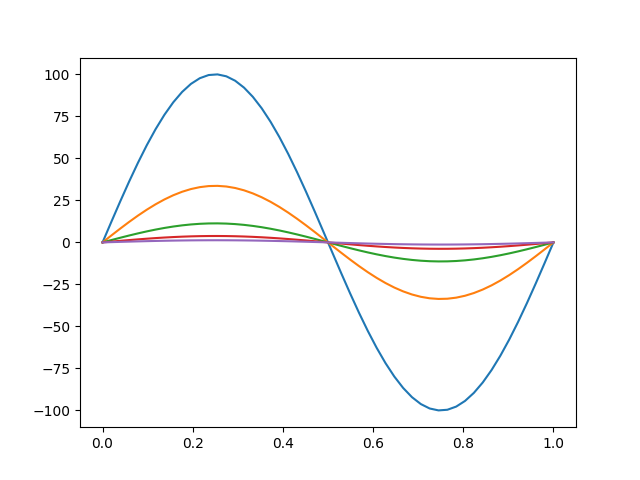
\includegraphics[width=7cm]{chaleurImplicite.png}
\end{center}
\end{frame}
  
   
  
  
  
 \begin{frame}    
  \frametitle{ Le schéma saute-mouton}
Tous les schémas imaginables ne sont pas nécessairement bons, comme le montre l'exemple suivant : on pourrait chercher à améliorer la précision en temps en utilisant l'approximation d'ordre 2 (voir section 2.1.1) suivante de la dérivée en temps :
\[\frac{\partial u}{\partial t}(x_i,t_j) \simeq \frac{u(x_{i},t_{j+1})-u(x_{i},t_{j-1})}{2\Delta t}\simeq
\frac{u_{i}^{(j+1)}-u_{i}^{(j-1)} }{2\Delta t}\]
On obtiendrait alors le schéma
 \begin{equation}
   \frac{U^{(j+1)}-U^{(j-1)} }{2\Delta t} +A_h^{(0)}U^{(j)} =C^{(j)} , \quad \forall j\in\{2,...,m-1\} 
   \end{equation}
 qui est explicite en temps, puisque $U^{(j+1)}$ s'exprime directement en fonction de $U^{(j)}$ et $U^{(j-1)}$. On note qu'il est nécessaire pour ce schéma de connaître U(0) et U(1). Le précalcul de $U^{(1)}$ peut par exemple être fait en utilisant un pas en temps de l'une des méthodes précédentes.
 
Ce schéma, appelé schéma saute-mouton ou schéma de Richardson, est à la fois explicite et a priori d'ordre 2 en temps. Cependant, comme on le verra plus loin, il est toujours instable, et donc numériquement inutilisable.
  \end{frame}
  
  \begin{frame}    
  \frametitle{Consistance, stabilité et convergence}
  Les trois schémas précédents peuvent s'écrire sous la forme générale
  \[B_1U^{(j+1)} + B_0U^{(j)} + B_{-1}U^{(j-1)} = C^{(j)}\]
  avec $B_1$ inversible ou $B_1 = 0$ et $B_0$ inversible. Pour le schéma explicite, on a
\[B_1= \frac{1}{\Delta t} Id,\quad B_0=-\frac{1}{\Delta t} Id+A_h^{(0)},\quad  B_{-1}=0.\]
Pour le schéma implicite, on a
 \[B_1= 0,\quad B_0=\frac{1}{\Delta t} Id+A_h^{(0)},\quad  B_{-1}=-\frac{1}{\Delta t} Id.\]
Pour le schéma suate-mouton, on a

\[B_1= \frac{1}{\Delta t} Id ,\quad B_0=A_h^{(0)},\quad  B_{-1}=-\frac{1}{\Delta t} Id.\]

L'étude de la convergence de ces schémas est basée sur les propriétés de consistance et stabilité, définies ci-dessous pour le schéma général .
On pourrait bien sûr imaginer des schémas faisant intervenir des indices en temps plus grands que $j + 1$ et plus petits que $j - 1$. Les définitions suivantes s'étendraient sans difficulté à ces schémas.

  
  \end{frame}
  
  \begin{frame}    
  \frametitle{Définition}
  On appelle erreur de consistance à l'instant $t_j$:
  \[\varepsilon_h(u)^{(j)} = B_1(\pi_h(u))(t_{j+1})+B_0(\pi_h(u))(t_{j})+B_{-1}(\pi_h(u))(t_{j-1})-C^{(j)},\]
  où
  \[\pi_h(u)(t) = \left( \begin{array}{c}
  u(t,x_1)\\
  \vdots\\
  u(t,x_N)
  \end{array}\right)
  \]
  On dit que le schéma est consistant pour la norme $\|\cdot\|$ de $\mathbb{R}^N$ si
  \[\sup_{0\leq j \leq M+1}\|\varepsilon_h(u)^{(j)} \|\to 0,\quad\mbox{ quand }\quad \Delta t\to 0 \mbox{ et }h\to 0.\]
  Si de plus il existe $C>0$, $p>0$ et $q>0$ indépendants de $\Delta t$ et $h$ tels que
  \[\sup_{0\leq j \leq M+1}\|\varepsilon_h(u)^{(j)} \|\leq C\left[(\Delta t)^p +h^q\right],\]
  On dir que le schéma est consistant d'ordre $p$ en temps et $q$ en espace pour la norme  $\|\cdot\|$ .
   \end{frame}
   
   \begin{frame}    
  \begin{block}{Proposition}
  Supposons que la solution $u$ au problème de la chaleur est $C^2$ par rapport à la variable t et $C^4$ par rapport à la variable $x$. Alors les schémas explicites et implicites sont consistants d'ordre 1 en temps et 2 en espace.
Si de plus $u$ est $C^3$ par rapport à la variable t, alors le schéma saute-mouton est consistant d'ordre 2 en temps et en espace.
  \end{block}
  On a $f(t_j,x_i)=\frac{\partial u}{\partial t}(t_j,x_i)-\frac{\partial^2 u}{\partial x^2}(t_j,x_i)$, On pose
  \[\varepsilon_h(u)^{(j)} =E_i-F_i\]
  où
  \[\begin{array}{l}
E_i=\frac{u(t_{j+1},x_i)-u(t_j,x_i)}{\Delta t}  -\frac{\partial u}{\partial t}(t_j,x_i),\\
F_i=\frac{u(t_{j},x_{i+1})-2u(t_j,x_i)+u(t_{j},x_{i-1})  }{h^2}-\frac{\partial^2 u}{\partial x^2}(t_j,x_i)
  \end{array}
  \]
  Par développement de Taylor:
  \[u(t_{j+1},x_i)=u(t_{j},x_i)+\Delta t  \frac{\partial u}{\partial t}(t_j,x_i) + \frac{\Delta t^2}{2}\frac{\partial^2 u}{\partial t^2}(\theta,x_i)\]
  \end{frame}
   
   \begin{frame}    
  D'où
  \[E_i=\frac{\Delta t}{2}\frac{\partial^2 u}{\partial t^2}(\theta,x_i)\]
De même
 \[F_i=\frac{h^2}{2}\left(\frac{\partial^4 u}{\partial t^4}(t_j,\xi_1)+\frac{\partial^4 u}{\partial t^4}(t_j,\xi_2)\right)\]
 \begin{block}{Définition}
 On dit que le schéma
  \[B_1U^{(j+1)} + B_0U^{(j)} + B_{-1}U^{(j-1)} = C^{(j)}\]
  est convergent ssi
  \[ \sup_{0\leq j \leq M+1}\|U^{(j)}-(\pi_hu)(t_j)\|\to 0\quad \mbox{ quand } \Delta t \mbox{ et } h\to 0\]
  \end{block}
   \end{frame}
   
    \begin{frame}    
 \begin{block}{Définition}
 On dit que le schéma
  \[B_1U^{(j+1)} + B_0U^{(j)} + B_{-1}U^{(j-1)} = C^{(j)}\]
  est stable ssi il existe deux constante $C_1(T)$ et $C_2(T)$ telles que
  \[ \max_{0\leq j \leq M+1}\|U^{(j)}\|\leq C_1(T) \|U^{(0)}\| + C_1(T)\max_{0\leq j \leq M+1} \|C^{(j)}\| \]
  \end{block}
  
   \begin{block}{Théorème de Lax}
 Le schéma
  \[B_1U^{(j+1)} + B_0U^{(j)} + B_{-1}U^{(j-1)} = C^{(j)}\]
  converge ssi il est  stable et consistant.
   \end{block}
  
   \end{frame}
   
   \begin{frame}    
 \begin{block}{Proposition}
 Sous la condition \[\frac{\Delta t}{h^2}\leq \frac 12\]
 Le schéma explicite converge.
  \end{block} 
   \end{frame}
   %%%%%%%%%%%%%%%%%%%%%%%%%%%%%%%%%%%%%%%%%%%%%%%%%%%%%%%%%%%%%%%%%%%%%%%
%%%%%%%%%%%%%%%%%%%%%%%%%%%%%%%%%%%%%%%%%%%%%%%%%%%%%%%%%%%%%%%%%%%%%%% 
    \begin{frame}  
    \frametitle{Équation d'advection}
    \[\myredbox{\left\{\begin{array}{ll}
    \displaystyle \frac{\partial u}{\partial t} +V \frac{\partial u}{\partial x}  = 0 & \forall(x,t)\in [0,1]\times \mathbb{R}^+\\
    u(x+1,t)=u(x,t) & \forall(x,t)\in \mathbb{R}\times \mathbb{R}^+\\ 
    u(x,t=0)=u_0(x) & \forall(x,t)\in [0,1]
    \end{array}\right.}\]
    
On va étudier l'équation aux dérivées partielles suivante :
où $V$ est un réel non nul.


 \begin{block}{Remarque}
  Cette équation, aussi appelée équation de transport, intervient par exemple dans l'étude du transport d'un polluant
dans un courant d'un fluide. 

$V$ est alors à interpréter comme la vitesse du courant. Noter qu'on peut avoir $V>0$ ou $V< 0$ en fonction du sens du courant.
\end{block}
\end{frame}

%%%%%%%%%%%%%%%%%%%%%%%%%%%%%%%%%%%%%%%%%%%%%%%%%%%%%%%%%%%%%%%%%%%%%%%
%%%%%%%%%%%%%%%%%%%%%%%%%%%%%%%%%%%%%%%%%%%%%%%%%%%%%%%%%%%%%%%%%%%%%%% 
\begin{frame}  
\frametitle{Équation d'advection}
 Dans le cas de ce problème simple, l'expression de la solution est
connue. La solution s'écrit
    \[\myredbox{u(x, t) = u_0(x-V t)}\]
En effet, on aura $\frac{\partial u}{\partial x} =u'_0(x-V t) $ et
$\frac{\partial u}{\partial t} -V u'_0(x-Vt)$ et donc bien 
$\frac{\partial u}{\partial t} +V \frac{\partial u}{\partial x}  = 0$


 \begin{block}{Remarque}
On a choisi ici des conditions aux limites de périodicité, mais on aurait pu envisager d'autres types de conditions aux limites. Il faudrait en tenir compte pour le traitement des équations aux bords de l'intervalle d'espace.
\end{block}
\end{frame}

%%%%%%%%%%%%%%%%%%%%%%%%%%%%%%%%%%%%%%%%%%%%%%%%%%%%%%%%%%%%%%%%%%%%%%%
%%%%%%%%%%%%%%%%%%%%%%%%%%%%%%%%%%%%%%%%%%%%%%%%%%%%%%%%%%%%%%%%%%%%%%% 
\begin{frame}  
\frametitle{Équation d'advection}
Discrétisation
Posons $h =\frac 1N$ pour discrétiser l'intervalle d'espace.

On a donc $x_j=jh$  et en particulier $x_0=0$, $x_N=1$.

On pose $t_n=n\tau$  avec $\tau$  le pas de temps.

Ainsi, on posera comme inconnue discrète à chaque pas de temps
le vecteur
\[u^{(n)} = \left(\begin{array}{c}
u_0^{(n)}  \\ u_1^{(n)} \\ \vdots \\ u_{N-1}^{(n)} 
\end{array}\right)\]
La condition de périodicité se traduira par $u_N^{(n)} =u_0^{(n)} $.

On considère aussi $u_{N-1}^{(n)} =u_{-1}^{(n)} $.
\end{frame}

%%%%%%%%%%%%%%%%%%%%%%%%%%%%%%%%%%%%%%%%%%%%%%%%%%%%%%%%%%%%%%%%%%%%%%%
%%%%%%%%%%%%%%%%%%%%%%%%%%%%%%%%%%%%%%%%%%%%%%%%%%%%%%%%%%%%%%%%%%%%%%% 
\begin{frame}  
\frametitle{Équation d'advection: Discrétisation}

Posons $h =\frac 1N$ pour discrétiser l'intervalle d'espace.

On a donc $x_j=jh$  et en particulier $x_0=0$, $x_N=1$.

On pose $t_n=n\tau$  avec $\tau$  le pas de temps.

Ainsi, on posera comme inconnue discrète à chaque pas de temps
le vecteur
\[u^{(n)} = \left(\begin{array}{c}
u_0^{(n)}  \\ u_1^{(n)} \\ \vdots \\ u_{N-1}^{(n)} 
\end{array}\right)\]
La condition de périodicité se traduira par $u_N^{(n)} =u_0^{(n)} $.

On considère aussi $u_{N-1}^{(n)} =u_{-1}^{(n)} $.
\end{frame}

%%%%%%%%%%%%%%%%%%%%%%%%%%%%%%%%%%%%%%%%%%%%%%%%%%%%%%%%%%%%%%%%%%%%%%%
%%%%%%%%%%%%%%%%%%%%%%%%%%%%%%%%%%%%%%%%%%%%%%%%%%%%%%%%%%%%%%%%%%%%%%% 
\begin{frame}  
\frametitle{Équation d'advection: Schéma explicite centré}
\[\frac{u_j^{(n+1)}-u_j^{(n)}}{\tau}-\frac{u_{j+1}^{(n)}-u_{j-1}^{(n)}}{2h}=0\quad
(n\geq 0, \; 0\leq j\leq N-1)\]

Un schéma possible serait le schéma explicite centré :
\[u_j^{(n+1)}=\frac{c}{2}u_{j-1}^{(n)}+u_j^{(n)}-\frac{c}{2}u_{j+1}^{(n)}\quad \mbox{ avec } c=\frac{V\tau}{h}\]
Ce schéma pourrait se formuler ainsi :
\end{frame}

%%%%%%%%%%%%%%%%%%%%%%%%%%%%%%%%%%%%%%%%%%%%%%%%%%%%%%%%%%%%%%%%%%%%%%%
%%%%%%%%%%%%%%%%%%%%%%%%%%%%%%%%%%%%%%%%%%%%%%%%%%%%%%%%%%%%%%%%%%%%%%% 
\begin{frame}  
\frametitle{Équation d'advection: Schéma explicite centré}
Et donc une formulation matricielle de la forme 
\[ u^{(n+1)} = M u^{(n)}\]
avec
\[M=\left(\begin{array}{ccccccc}
1 & -\frac c2 & 0 & 0 & 0 & \cdots & \frac c2\\
\frac c2 &1 & -\frac c2 & 0 & 0 &   \cdots & 0\\
0 & \frac c2 &1 & -\frac c2 & 0 &   \cdots & 0\\
\vdots & \vdots & \vdots & \ddots & \ddots & \ddots & \vdots  \\
-\frac c2 &0 & 0 & 0 & 0 &   \cdots & 1\\
\end{array}\right)\]

en tenant de la condition de périodicité.
\end{frame}


%%%%%%%%%%%%%%%%%%%%%%%%%%%%%%%%%%%%%%%%%%%%%%%%%%%%%%%%%%%%%%%%%%%%%%% 
\begin{frame}  
\frametitle{Propriétés du schéma explicite centré}



 \begin{block}{Lemme}
Le schéma explicite centré est consistant avec l'équation
d'advection ci-dessus, précis à l'ordre 1 en temps et 2 en espace,
\end{block}
\end{frame}



%%%%%%%%%%%%%%%%%%%%%%%%%%%%%%%%%%%%%%%%%%%%%%%%%%%%%%%%%%%%%%%%%%%%%%%
%%%%%%%%%%%%%%%%%%%%%%%%%%%%%%%%%%%%%%%%%%%%%%%%%%%%%%%%%%%%%%%%%%%%%%% 
\begin{frame}  
\frametitle{Équation d'advection: Exemple}

On considère l'équation d'advection suivante:
$$ \left\{ 
    \begin{array}{l}
\displaystyle \frac{\partial u}{\partial t}+ 3\frac{\partial u}{\partial x}=0, \quad 0\leq x\leq 1,\quad t \in \mathbb{R}^+\\
u(x+1,t)=u(x,t)\\
u(x,0)=u_0(x)= \cos(\pi x)^8
    \end{array}  
    \right. 
  $$

\end{frame}

%%%%%%%%%%%%%%%%%%%%%%%%%%%%%%%%%%%%%%%%%%%%%%%%%%%%%%%%%%%%%%%%%%%%%%%


\begin{frame}[fragile]   
\begin{minted}[
mathescape,
framesep=2mm,
baselinestretch=1.2,
%fontsize=\footnotesize,
bgcolor=LightGray,
%linenos
]{python}
import matplotlib.pyplot as plt
import numpy as np

# Initialisation des constantes
h=0.005; tau=0.0002
nu = 3.0;c = nu * tau / h
N = int(1 / h)
nmax = int(1 / tau)

# Coordonnées en espace
X = np.linspace(0, 1, N + 2)[:-1]

# Initialisation temporelle
t = np.linspace(0, 1, nmax + 1)
\end{minted}

\end{frame}

\begin{frame}[fragile]   
\begin{minted}[
mathescape,
framesep=2mm,
baselinestretch=1.2,
%fontsize=\footnotesize,
bgcolor=LightGray,
%linenos
]{python}
# Initialisation de la solution
U = np.zeros((nmax + 1, N + 1))
U[0, :] = (np.cos(np.pi * X)) ** 8
# Matrice de taille N-N
M=np.eye(N+1)+c/2*np.diag(np.ones(N),1)
                        -c/2*np.diag(np.ones(N),-1)
M[0,N]=-c/2
M[N,0]=c/2
for n in range(nmax):
    U[n + 1,:] = np.dot(M, U[n,:])
K=nmax//10
for i in range(nmax//K):
    plt.plot(X, U[K*i,:], label = 'explicite centre')
plt.show()
\end{minted}
\end{frame}

\begin{frame}
 \begin{center}
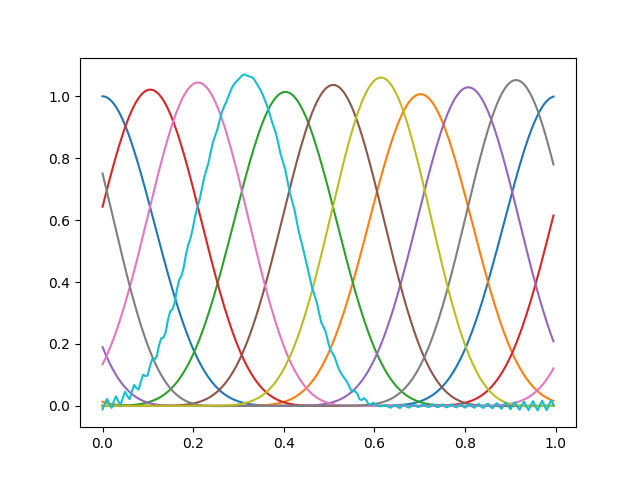
\includegraphics[width=7cm]{advection.png}
\end{center}
\end{frame}


\end{document}
   

























